\section*{DATA}\label{data}
The data used in this study is described in
Tab.\ref{fig:data_description}.
\begin{figure}[H]
\begin{center}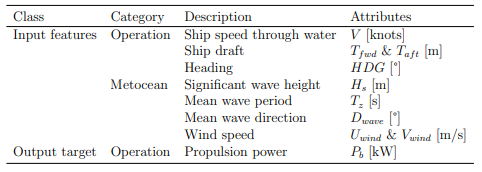
\includegraphics[width = 0.95\textwidth]{figures/data_description.png}\end{center}
\vspace{-0.7cm}
\caption{Spring-mass-damper system}
\label{fig:data_description}
\end{figure}
\subsection*{Exploratory data analysis}\label{exploratory-data-analysis}
The ship speed $V$, ship draughts $T_{aft}$ and $T_{fwd}$ were all
negative in the raw data file. This was imidiatelly corrected, to be
more in line with what would be expected from a more general sign
convention. The data seems to have been collected in time cronological
order, giving a time series of data. For a time series, measurements
close to each other in time have a high correlation, as they are
experiencing similar envinronmental conditions etc. This is confirmed by
looking at the autocorrelation plot in
Fig.\ref{fig:power_autocorrelation}. Dead reckoning (using ship
speed and heading) has been used to atempt to describe motion of the
ship as seen in Fig.\ref{fig:dead_reckoning}. The positions are
given in an unknown logintude and latitude scale, as the time step
between measurements is unknown. The speed of the ship is also indicated
as a color gradient in this figure.
\begin{figure}[H]
\begin{center}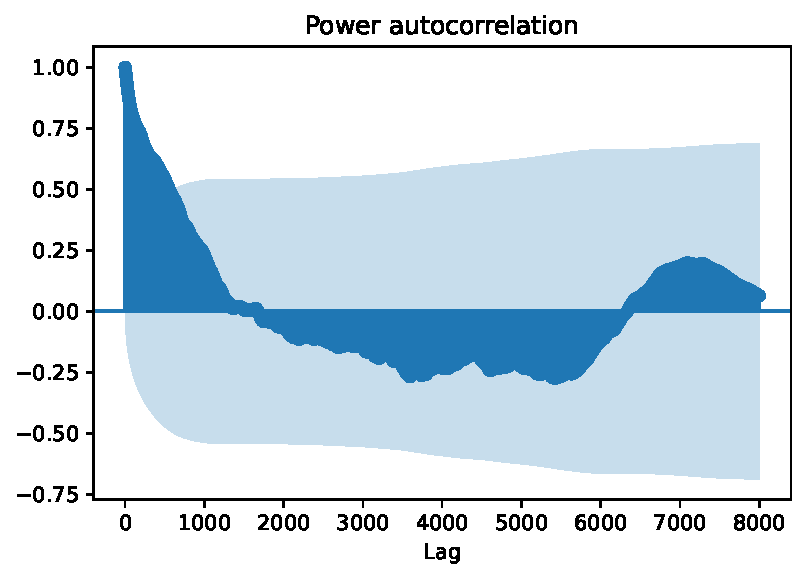
\includegraphics[width = 0.95\textwidth]{figures/power_autocorrelation.pdf}\end{center}
\vspace{-0.7cm}
\caption{Autocorrelation plot of the Power data}
\label{fig:power_autocorrelation}
\end{figure}
\begin{figure}[H]
\begin{center}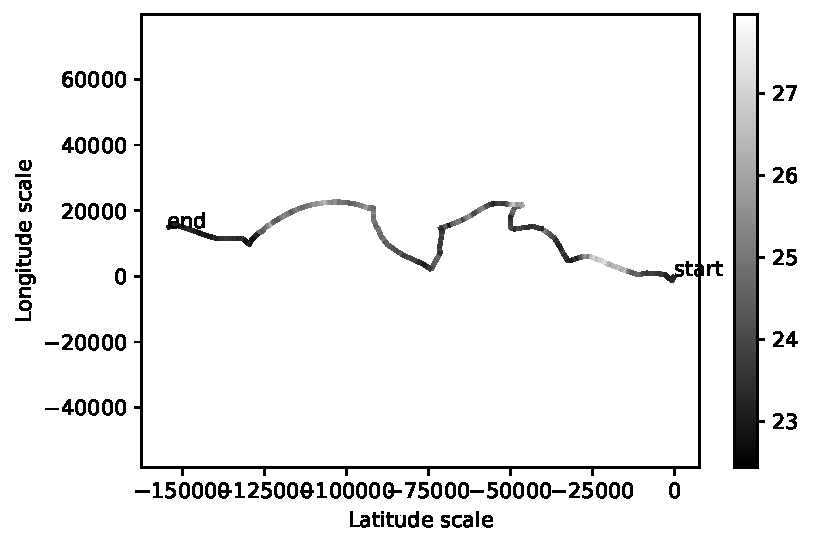
\includegraphics[width = 0.95\textwidth]{figures/dead_reckoning.pdf}\end{center}
\vspace{-0.7cm}
\caption{Dead reckoning of the position of the ship}
\label{fig:dead_reckoning}
\end{figure}
Fig.\ref{fig:heat_map_raw_data} shows a heat map of the absolute
linear correlation coefficient between all of the features in the raw
data. It can be seen that $T_{aft}$ and $T_{fwd}$ have the highest
correlation with the $Power$. It can also be seen that the correlation
between $T_{aft}$ and $T_{fwd}$ is also very high (approximately 1)
implying a very high multicollinearity which is generally something that
should be avoided in regression problems. These two features are instead
replaced with the two features: mean draught $T$ and $trim$. The
correspondig heat map with the new features is shown in
Fig.\ref{fig:heat_map_data}. The mean draught $T$ now seems to
be a very important feature in this regression as it has the highest
linear correlation with the $Power$. This can also be seen in
Fig.\ref{fig:power_draught}, where the $Power$ has been
plotted together with the corresponding negative draught.
\begin{figure}[H]
\begin{center}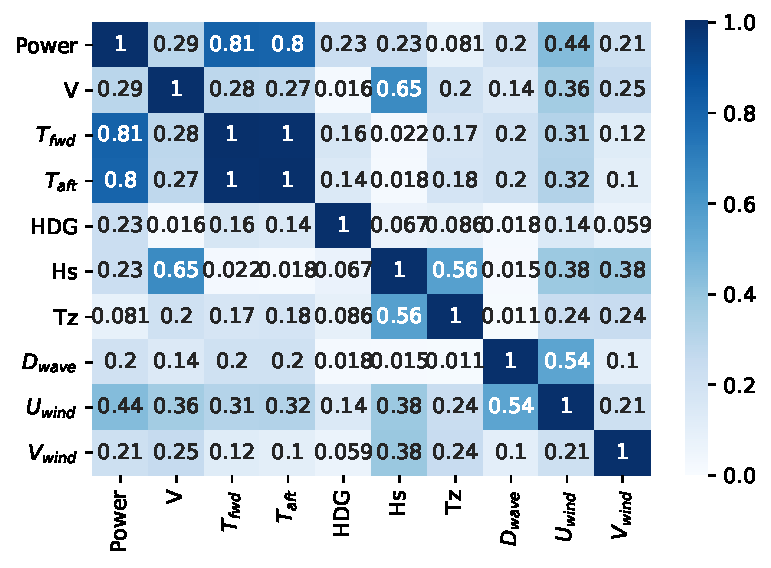
\includegraphics[width = 0.95\textwidth]{figures/heat_map_raw_data.pdf}\end{center}
\vspace{-0.7cm}
\caption{Heat map showing absolute value of correlation coefficient between features in raw data}
\label{fig:heat_map_raw_data}
\end{figure}
\begin{figure}[H]
\begin{center}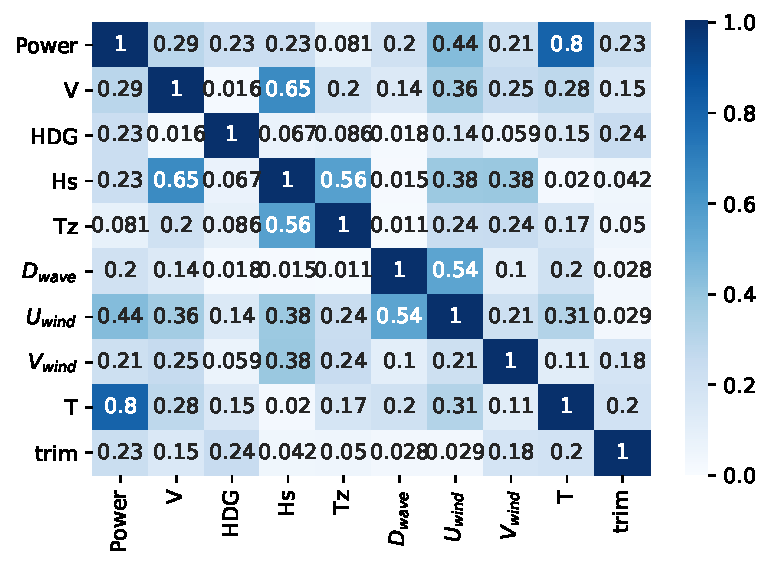
\includegraphics[width = 0.95\textwidth]{figures/heat_map_data.pdf}\end{center}
\vspace{-0.7cm}
\caption{Heat map showing absolute value of correlation coefficient between features in transformed data}
\label{fig:heat_map_data}
\end{figure}
\begin{figure}[H]
\begin{center}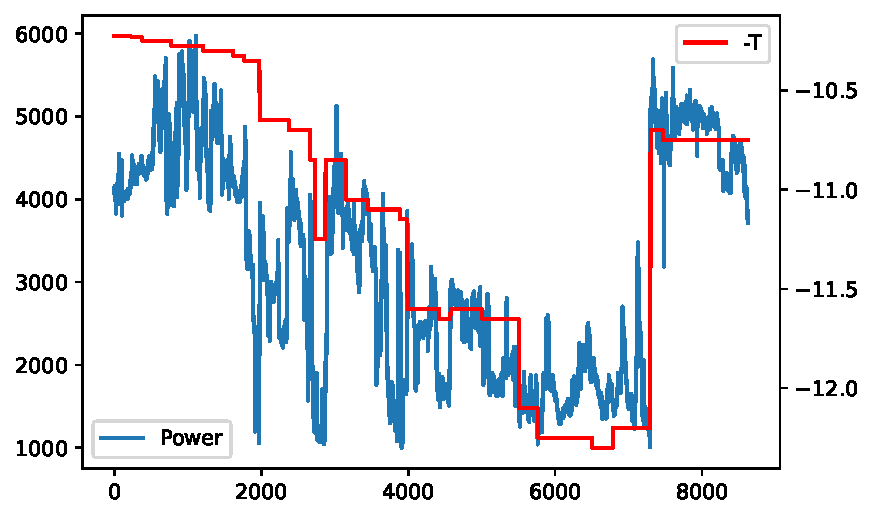
\includegraphics[width = 0.95\textwidth]{figures/power_draught.pdf}\end{center}
\vspace{-0.7cm}
\caption{The power is highly correlated with the draught}
\label{fig:power_draught}
\end{figure}
\subsection*{Extend data}\label{extend-data}
The data has also been extended by adding some additional features,
describing the wind speed and wave direction in a ship fixed coordinate
system:$u_{wind}$, $v_{wind}$, $wave_{direction}$. The new
features have very low linear correlation with $Power$ as seen in
Fig.\ref{fig:heat_map_extended_data}. They are however kept in
the data, to let the regression model decide if they are useable or not.
\begin{figure}[H]
\begin{center}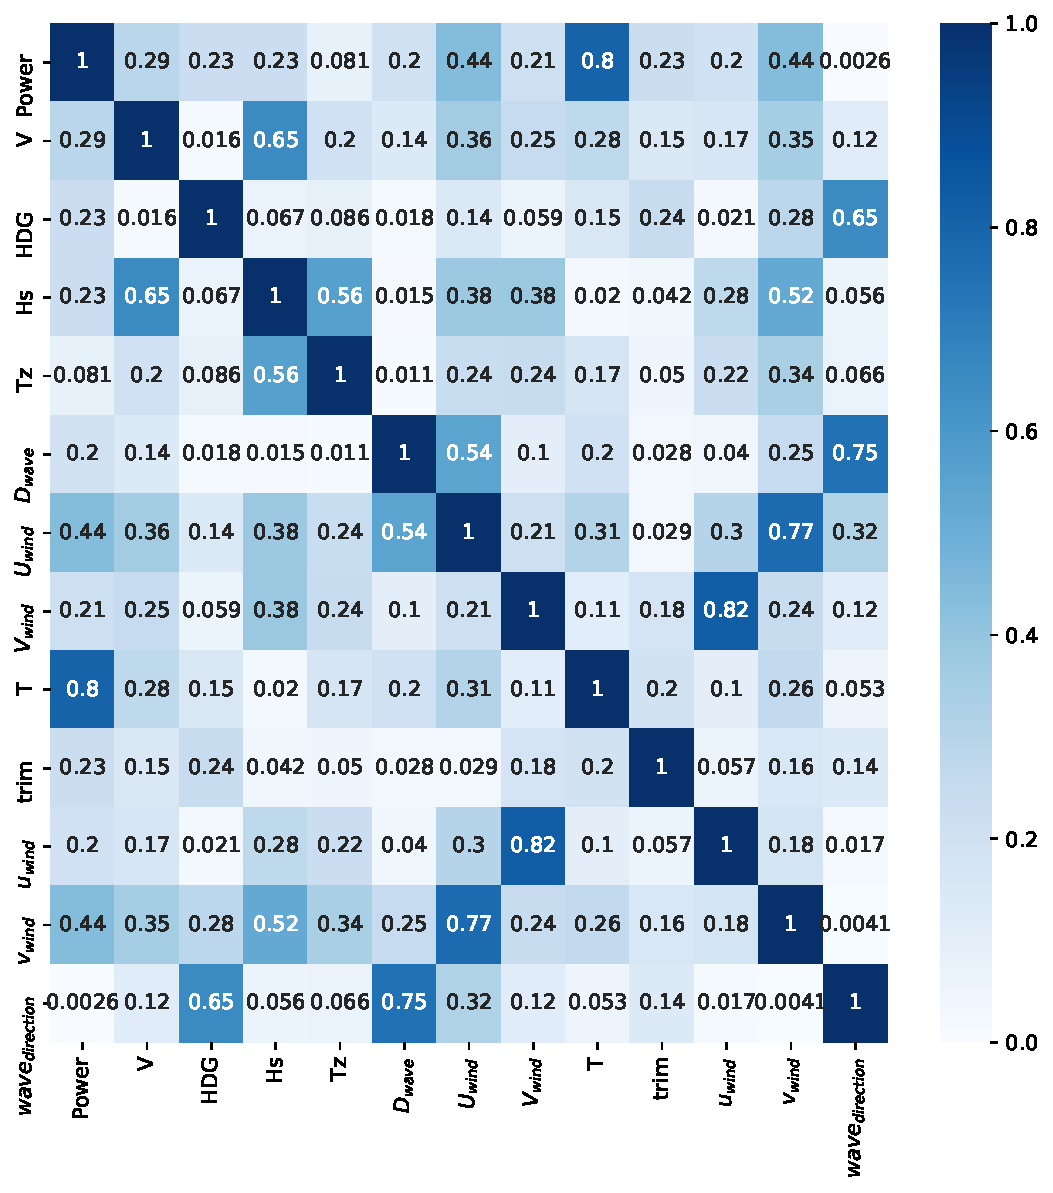
\includegraphics[width = 0.95\textwidth]{figures/heat_map_extended_data.pdf}\end{center}
\vspace{-0.7cm}
\caption{Heat map of data with additional features.}
\label{fig:heat_map_extended_data}
\end{figure}
